\documentclass[11pt,letterpaper]{article}
\usepackage[margin=.65in,top=.78in,bottom=.65in]{geometry}
\usepackage[T1]{fontenc}
\usepackage{lmodern,tikz,array,fancyhdr}
\usetikzlibrary{arrows.meta}
\renewcommand{\familydefault}{\sfdefault}
\pagestyle{fancy}\fancyhf{}
\fancyhead[L]{\small Week 75 / Twists on a cylinder / Grades 4--5}
\fancyfoot[L]{\small Bellingham Math Circle / Week 75 / GGT75-S-v1}
\fancyfoot[R]{\small\thepage}
\renewcommand{\headrulewidth}{0pt}\renewcommand{\footrulewidth}{0pt}
\setlength{\parindent}{0pt}\setlength{\parskip}{8pt}
\newcommand{\problem}[2]{\textbf{Problem #1:} #2\par}
\newcommand{\answerline}{\par\vspace{.32in}\hrule height .25pt}
\newcommand{\liftboard}{\begin{center}\begin{tikzpicture}[x=1.55in,y=1.3in,font=\small]
\draw[thick](-1,0)rectangle(3,1);
\foreach\k in {0,1,2}{\draw[dashed](\k,0)--(\k,1);}
\foreach\k in {-1,0,1,2}{\fill(\k+.5,1)circle(1.5pt);\node[above]at(\k+.5,1){B, copy \k};}
\fill(.5,0)circle(2pt)node[below]{A, start};
\end{tikzpicture}\end{center}}
\begin{document}
Keep the cylinder still. Each yarn route goes upward from A to B, with no self-crossings. Except at A and B, keep the yarn strictly between the rims. Leave spare yarn past both marks. Tape it at A and B; feed spare yarn through if needed, keeping the marked endpoints fixed. To build a different route, lift and re-lay the yarn, putting its ends back on the same marks.

Travel from A to B. At the seam, a rightward crossing counts $+1$; a leftward crossing counts $-1$. Add these to get the route's \emph{winding}.
\begin{center}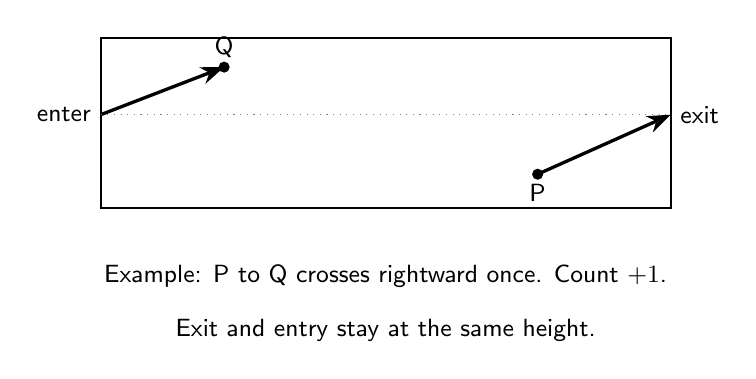
\begin{tikzpicture}[x=.95in,y=.85in,font=\small,>=Stealth]
\draw[thick](0,0)rectangle(3,1);
\draw[dashed](0,0)--(0,1);\draw[dashed](3,0)--(3,1);
\draw[very thick,->](2.3,.2)--(3,.55);
\draw[very thick,->](0,.55)--(.65,.83);
\fill(2.3,.2)circle(2pt)node[below]{P};\fill(.65,.83)circle(2pt)node[above]{Q};
\draw[gray,dotted](0,.55)--(3,.55);
\node[left]at(0,.55){enter};\node[right]at(3,.55){exit};
\node at(1.5,-.4){Example: P to Q crosses rightward once. Count $+1$.};
\node at(1.5,-.72){Exit and entry stay at the same height.};
\end{tikzpicture}\end{center}
\problem{1}{Cut out the rectangle and tape its left and right edges together without overlap. Make yarn routes with winding 0, $+1$, $-1$ and $+2$. Your partner checks the seam crossings. Make two different-looking routes with the same winding.}
\vspace{.12in}
\begin{center}\begin{tikzpicture}[x=1in,y=1in,font=\small,>=Stealth]
\draw[dashed,thick](0,0)rectangle(6,2.4);
\draw[gray!45,dotted](0,.6)--(6,.6);\draw[gray!45,dotted](0,1.2)--(6,1.2);\draw[gray!45,dotted](0,1.8)--(6,1.8);
\fill(3,0)circle(2pt);\node[above]at(3,.02){A};\fill(3,2.4)circle(2pt);\node[below]at(3,2.38){B};
\node[rotate=90]at(.17,1.2){seam};\node[rotate=90]at(5.83,1.2){seam};
\draw[->,thick](4.6,1.3)--(5.35,1.3);\node[above]at(4.97,1.3){rightward};
\node at(1.35,.15){bottom rim};\node at(1.35,2.23){top rim};
\end{tikzpicture}\end{center}
\vspace{.15in}
Same winding, different routes: \hrulefill
\newpage
Instead of jumping back across the cut, continue into the next copy of the rectangle. The top dots are copies of the same B on the cylinder.
\begin{center}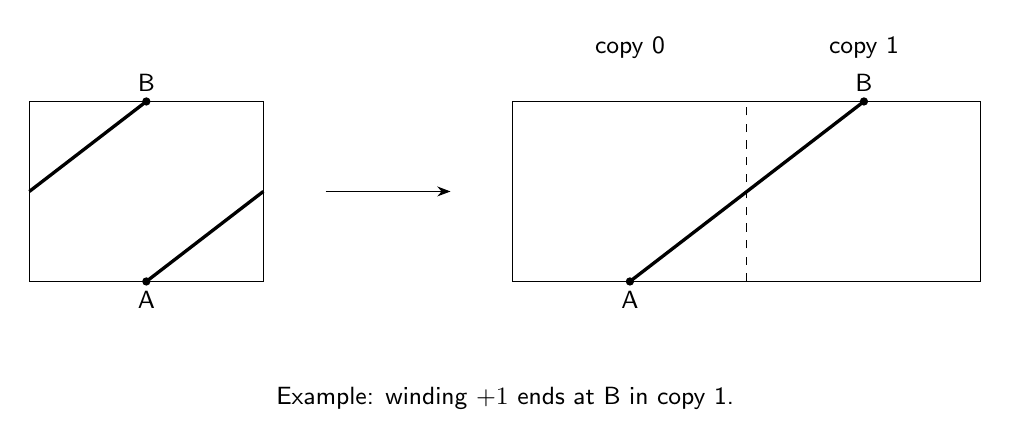
\begin{tikzpicture}[x=.78in,y=.9in,font=\small,>=Stealth]
\draw(0,0)rectangle(1.5,1);
\draw[very thick](.75,0)--(1.5,.5);\draw[very thick](0,.5)--(.75,1);
\fill(.75,0)circle(1.5pt)node[below]{A};\fill(.75,1)circle(1.5pt)node[above]{B};
\draw[->](1.9,.5)--(2.7,.5);
\draw(3.1,0)rectangle(6.1,1);\draw[dashed](4.6,0)--(4.6,1);
\draw[very thick](3.85,0)--(5.35,1);\fill(3.85,0)circle(1.5pt)node[below]{A};\fill(5.35,1)circle(1.5pt)node[above]{B};
\node at(3.85,1.3){copy 0};\node at(5.35,1.3){copy 1};
\node at(3.05,-.65){Example: winding $+1$ ends at B in copy 1.};
\end{tikzpicture}\end{center}
\problem{2}{Draw two different upward routes of winding $+2$, and two of winding $-1$. Start each at A. Your partner checks by tracing each route back onto the cylinder.}
\liftboard
\liftboard
\problem{3}{Choose two of your yarn routes. Keeping the endpoints at A and B and the yarn on the cylinder, can you slide one route into the other without crossing itself? Find a pair that can and a pair that cannot. Use the repeated rectangles to explain the difference.}
\answerline\answerline
\newpage
A $+$ twist moves points rightward: none at the bottom, a quarter-turn at the first dotted line, a half-turn at the middle, three-quarter-turns at the next line, and one full turn at the top. Between lines, the shift grows evenly. A $-$ twist uses the same shifts leftward.

Every rim point ends where it started. Draw the changed route and re-lay the yarn to match. The paper cylinder stays still.
\begin{center}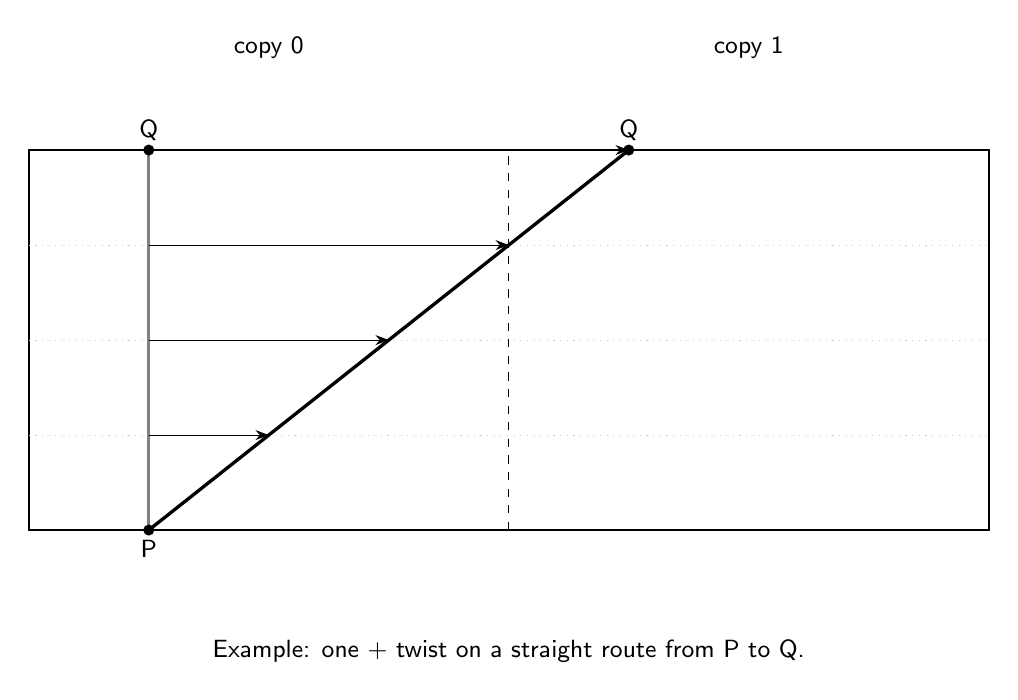
\begin{tikzpicture}[x=2.4in,y=1.9in,font=\small,>=Stealth]
\draw[thick](0,0)rectangle(2,1);\draw[dashed](1,0)--(1,1);
\foreach\h in {.25,.5,.75}{\draw[gray!40,dotted](0,\h)--(2,\h);}
\draw[gray,very thick](.25,0)--(.25,1);
\draw[very thick](.25,0)--(1.25,1);
\foreach\h in {.25,.5,.75,1}{\draw[->](.25,\h)--(.25+\h,\h);}
\fill(.25,0)circle(2pt)node[below]{P};\fill(.25,1)circle(2pt)node[above]{Q};\fill(1.25,1)circle(2pt)node[above]{Q};
\node at(.5,1.27){copy 0};\node at(1.5,1.27){copy 1};
\node at(1,-.32){Example: one $+$ twist on a straight route from P to Q.};
\end{tikzpicture}\end{center}
\problem{4}{Start with winding 0. Choose a secret word of two to four $+$ and $-$ twists. Make its final route. Your partner tries to make a route with the same winding using the fewest twists. Reveal your word and swap jobs. Which words have the same effect?}
\vspace{.1in}
\par\begin{tabular}{@{}p{.35\linewidth}p{.25\linewidth}p{.28\linewidth}@{}}
Secret word & Ending winding & Shortest word\\\hline
 & & \\[.28in]\hline
 & & \\[.28in]\hline
 & & \\[.28in]\hline
\end{tabular}\par
\vspace{.12in}
\problem{5}{Find a word of six twists that returns every starting route to its original winding. How can your partner check it without trying every possible starting route?}
\answerline\answerline
\newpage
\problem{6}{Lay two yarn routes from A to B with each pair of windings below. Make the number of crossings between the rims as small as possible. Your partner tries to remove another crossing without changing either winding.}

Both ends are shared. Do not count A or B. Away from the ends, the strands must cross or stay apart: no shared pieces or other touches.
\vspace{.12in}
\par\begin{tabular}{@{}p{.24\linewidth}p{.22\linewidth}p{.44\linewidth}@{}}
Windings & Fewest crossings & Sketch or seam-crossing record\\\hline
0 and 1 & & \\[.33in]\hline
0 and 2 & & \\[.33in]\hline
0 and 3 & & \\[.33in]\hline
$-1$ and 1 & & \\[.33in]\hline
$-1$ and 2 & & \\[.33in]\hline
2 and 4 & & \\[.33in]\hline
\end{tabular}\par
\vspace{.17in}
\problem{7}{Predict the fewest crossings for windings 2 and 7, then for 5 and 5. Find a rule for any pair of windings. Does adding the same twist to both routes change the fewest crossings? What can happen if you twist only one?}
\answerline\answerline\answerline
\end{document}
